\chapter{Introducción}

Presentar de forma atractiva el trabajo... 
Presentar los capítulos.


el título... All You Need is an AI Muse: Grandes modelos de lenguaje en la creación sonora.

<

% \begin{figure}[H]
%     \caption[Número de publicaciones de \textit{Deep Learning} por año que contienen la expresión <<all you need>> en el título]{Número de publicaciones de \textit{Deep Learning} por año que contienen la expresión <<all you need>> en el título.}
%     \centering
%     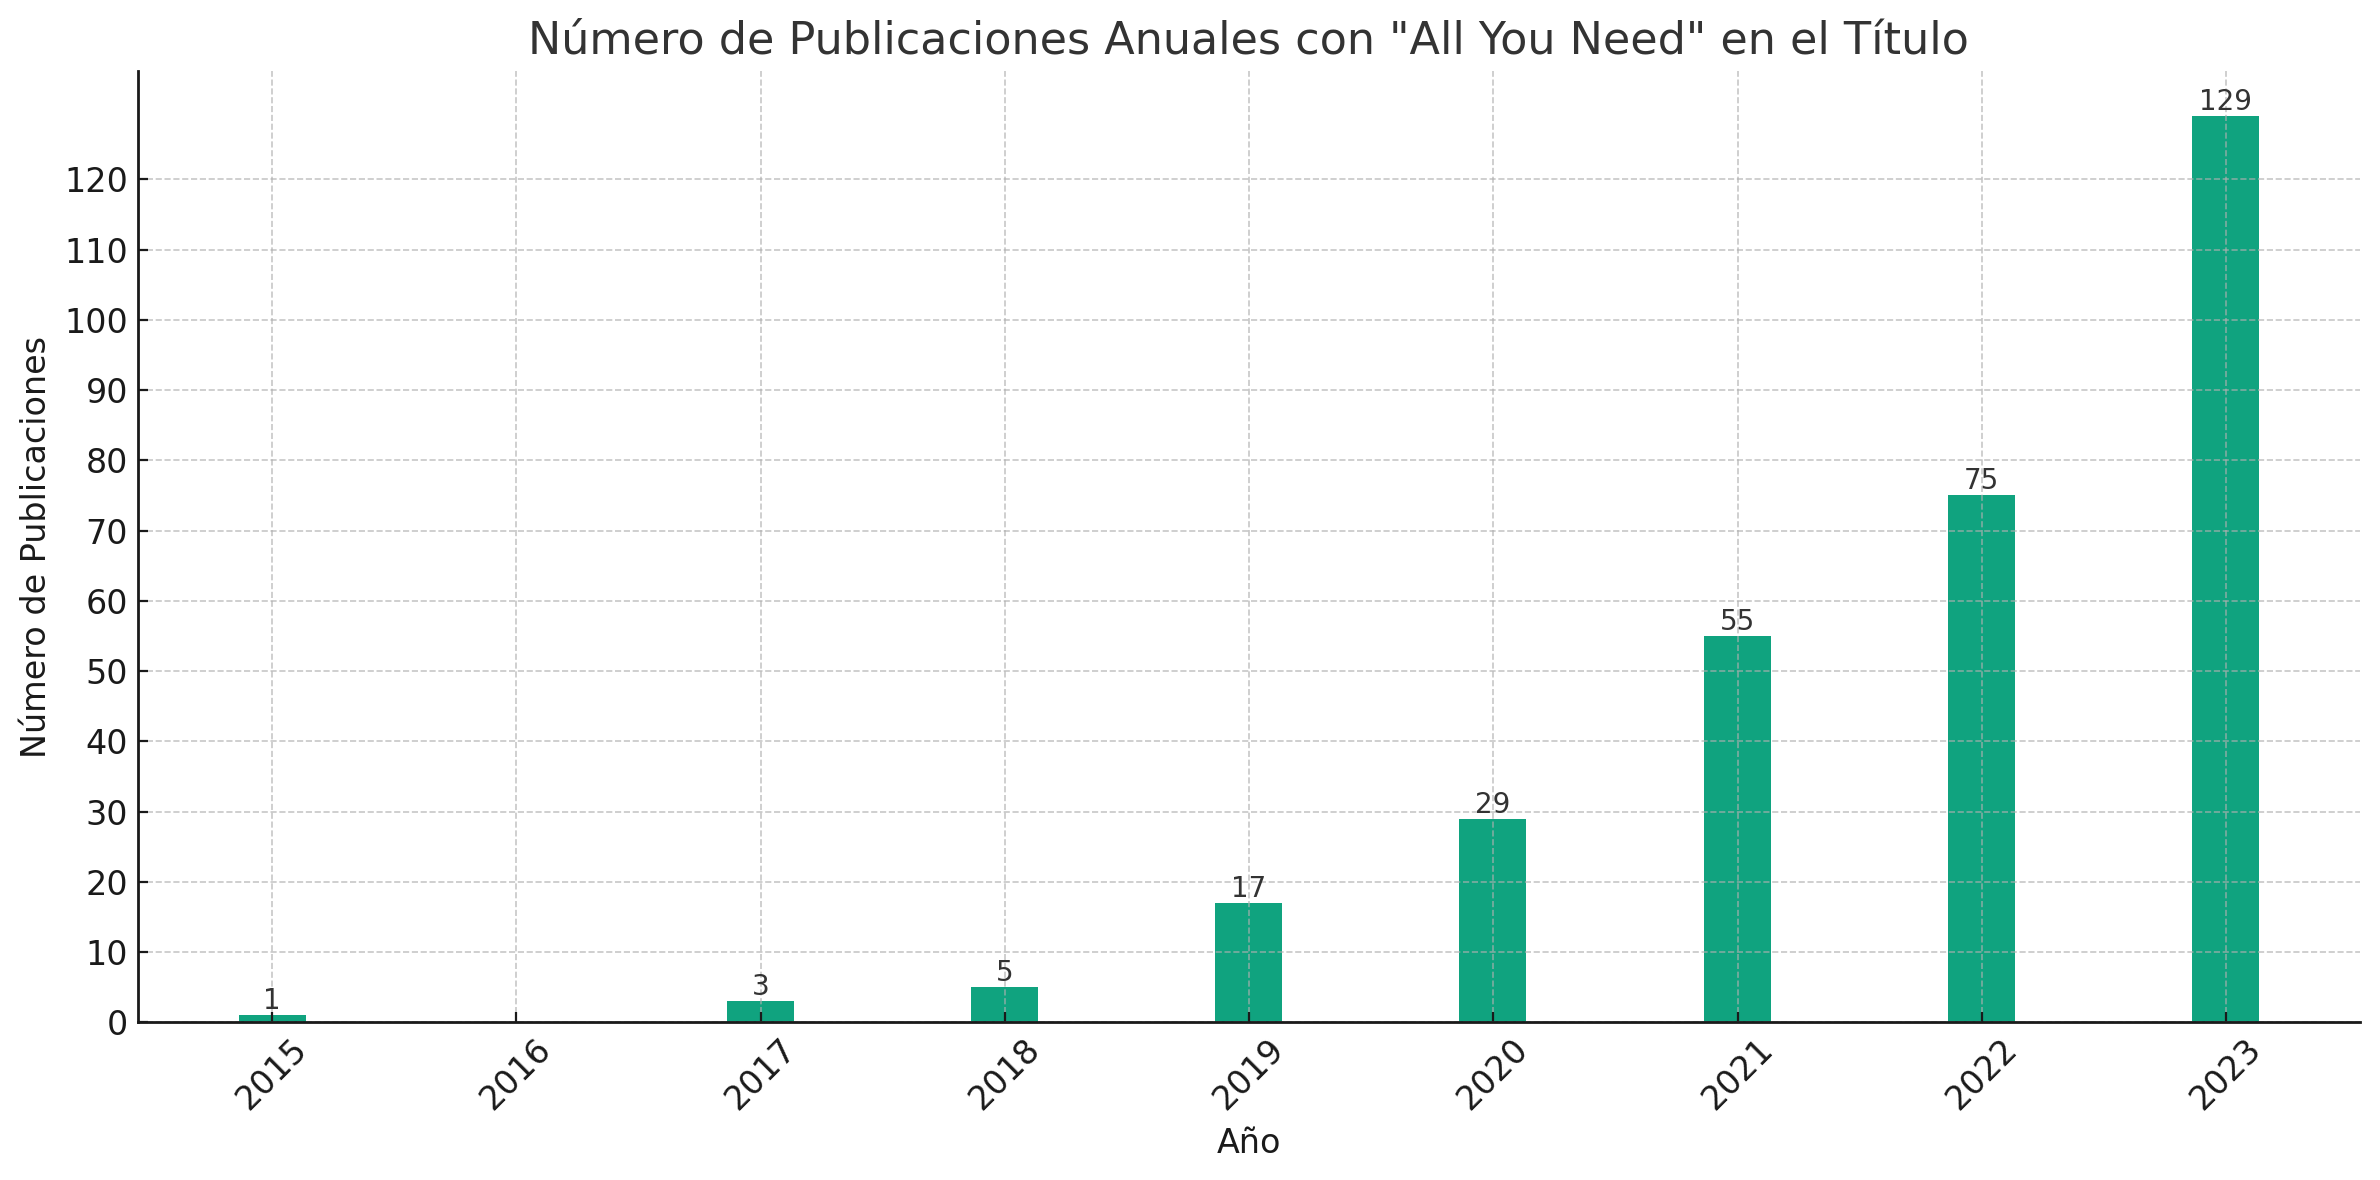
\includegraphics[width=0.9\textwidth]{./figuras/all_you_need_publicacionies_anuales.png}
%     \source{Elaboración propia a partir del listado de \url{https://github.com/KentoNishi/awesome-all-you-need-papers}}
%     \label{fig:all_you_need_publicaciones}
% \end{figure}




